\documentclass[a4paper]{article} %format de la feuille + type de document https://en.wikibooks.org/wiki/LaTeX/Document_Structure#Document_classes
%packages nécessaire pour nos besoins
\usepackage[utf8]{inputenc}
\usepackage[T1]{fontenc}
\usepackage[english,french]{babel}
\usepackage{amsmath}
\usepackage{amssymb,amsfonts,textcomp}
\usepackage{color}
\usepackage{array}
\usepackage{supertabular}
\usepackage{hhline}
\usepackage{hyperref}
\usepackage{capt-of}
\usepackage[pdftex]{graphicx}
\usepackage{sectsty}
\usepackage{tcolorbox}
\usepackage{textcomp}
\usepackage{courier}
\usepackage[font={small,it}]{caption}
\usepackage{float}
\usepackage{graphicx}
\usepackage{subcaption}
\usepackage{caption}


%Définition des couleurs
\definecolor{havelockBlue}{rgb}{0.004, 0.42, 0.73}
\definecolor{Monokaimagenta}{rgb}{0.86,0.08,0.24}

%utilisation de la couleur définie avant
%toutes les sections auront cette couleur
\sectionfont{\color{havelockBlue}}

%début du document
\begin{document}

%début d'un titre
\begin{titlepage}
            %centre les éléments
	\centering
	
	{\scshape\LARGE \color{Monokaimagenta} Laboratoire \\ Registres à décalage \par}
	
	%espace vertical de 1 mms
	\vspace{1cm}
	
	{\Large\itshape Johanna Melly \& Sven Rouvinez\par}
	
	%http://www.personal.ceu.hu/tex/spacebox.htm
	\vfill
	Professeur\par
	%met le texte en gras 
	\textbf{Carlos Andrés Pena} \par% ajoute une ligne 
	\vspace{1cm}
	Assistant\par
	\textbf{Gaëtan Matthey}
	
	\vfill

            %affiche la date actuelle
	{\large \today\par}
	
%fin de la page de titre
\end{titlepage}

%démarre un chapitre, les nombres se mettent automatiquement et seront incrémenté quand un autre \section est rencontré
%voir https://en.wikibooks.org/wiki/LaTeX/Document_Structure#Sectioning_commands
\section{Registre à décalage 4 bits}
Sur la base du registre à décalage vu dans le cours, concevoir et implémenter un registre à décalage de 4 bits qui peut décaler à gauche (SHL), décaler à droite (SHR), charger un nibble (LOAD) ou garder son contenu (HOLD). Le registre à décalage doit être réalisé à l’aide de flip-flops D et de multiplexeurs.\\%saut à la ligne


%début d'un encadré avec la couleur définie plus haut
\begin{tcolorbox}[colframe=Monokaimagenta,colback=white]
\paragraph{Registre à décalage 4 bits- Max 1 page } %démarre un paragraphe
Insérez une capture d’écran pour présenter votre bloc Registre à décalage 4 bits (Structure interne).
Accompagnez-le de commentaires et d’explications nécessaires à sa compréhension.
Remplacez le texte ci-dessus par vos réponses (à l’intérieur du cadre rouge)\\ 

\begin{figure}[H]
    \centering
    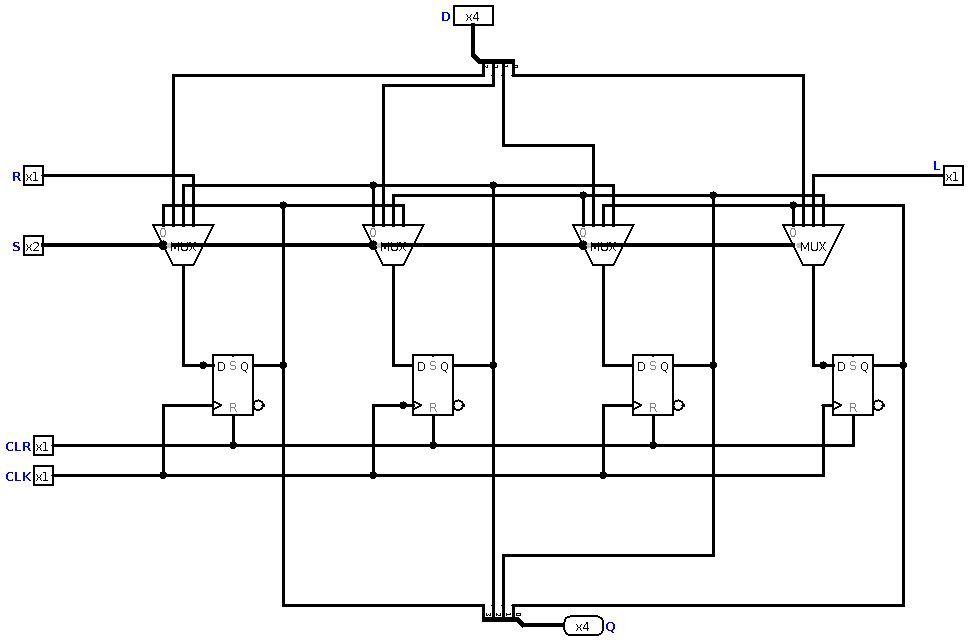
\includegraphics[width=.8\textwidth]{src/SHREGI_4BITS.png}
    \captionof{figure}{Bloc SHIFT REGISTER}
    \label{fig:SHREGI_4}
\end{figure}

Le registre à décalage 4 bits permet d'effectuer un décalage de tous les bits sur la droite ou sur la gauche. L'entrée \textbf{D} représente les bits qu'on veut pouvoir décaler.
L'entrée \textbf{S} permet de choisir l'action à effectuer: 
\begin{itemize}
    \item 00: HOLD, la valeur reste inchangée
    \item 01: LOAD, la valeur est placée dans l'état voulu
    \item 10: shift left, les bits sont tous décalés d'un cran verfs la gauche
    \item 11: shift right, les bits sont tous décalés d'un cran vers la droite
\end{itemize}
\vspace{1em}
L'entrée CLK est correspond à notre horloge, l'utilisation d'un entrée simple se justifie de la sorte que le bloc sera utilisé dans un autre cicruit qui lui aura une vraie horloge.\\
Lorsque l'horloge passe à 1 (flanc montant), la valeur des bits dans les balances sont changées, et lorsqu'elle passe à 0, la valeur des bits est conservée.
Ainsi, pout effectuer un décalage, il sera tout d'abord nécessaire de mettre l'entrée \textbf{S} à 1 et d'avoir un flanc montant pour que les bits des balances prennent la valeur de l'entrée \textbf{D}. Ensuite, on peut changer la valeur de l'entrée S dans le but d'avoir un décalage sur la droite ou sur la gauche. Dès lors, à chaque fois que l'horloge passera de 0 à 1, les bits vont tous se décaler d'un cran.
    
%fin de l'encadré
\end{tcolorbox}

\section{Registre à décalage 8 bits}\
Concevoir un registre à décalage de 8 bits en utilisant deux registres à décalage de 4 bits
\begin{tcolorbox}[colframe=Monokaimagenta,colback=white]
\paragraph{Registre à décalage 8 bits - Max 2 pages}
\paragraph
Insérez une capture d’écran pour présenter votre bloc Registre à décalage 8 bits (Structure interne).
Accompagnez-le de commentaires et d’explications nécessaires à sa compréhension.
Insérez une capture d’écran du chronogramme qui montre le chargement (Load) d’une valeur (exemple : 0x80), puis le décalage à droite de la valeur chargée (8 fois consécutif). 
Accompagnez le chronogramme d’explications.
Remplacez le texte ci-dessus par vos réponses (à l’intérieur du cadre rouge)\\
\paragraph
Le shift register 8 bits est composé de 2 shift register 4 bits.  Ils ont comme entrée en commun l'horloge CK, S qui détermine l'action à effectuer, ainsi que le reset. L'octet est séparé en deux nibbles qui sont chacun en entrée D des register 4 bits.
Lorsqu'un décalage est fait, le dernier bit d'un register doit être récupéré par le suivant, afin de ne pas perdre les bits décalés. Ainsi, pour le décalage à gauche, le bit [0] du shift register prenant en entrée D les bits [7:4] de l'octet (le SHREG\_I2 de l'illustration), doit être passé en entrée R de l'autre shift register (SHREGI\_1). Ainsi, au moment du décalage à gauche, le bit [0] du SHREGI\_2 va bien être passé au SHREGI\_1 et il y aura une continuité dans le décalage.
Le même principe est appliqué pour le décalage à droite, mais cette fois c'est le bit [3] du SHREGI\_1 qui va être donné en entrée L du SHREGI\_2.
\\
\end{tcolorbox}


\section {Générateur de nombres aléatoires}
Concevoir un générateur de nombres aléatoires à l’aide d’un registre LFSR (Linear Feedback Shift Register) 8-bits. Dans un registre LFSR Q+(n) = Q(n-1), n>1 et Q+(1) est la fonction XOR ou XNOR de plusieurs bits du registre. Notez que les bits du registre LFSR sont numérotés de 1 à n. Utilisez la documentation technique de Xilinx pour identifier les bits nécessaires pour calculer le bit Q+(1) et simuler le registre LFSR 8-bits à l’aide de Logisim.
\begin{tcolorbox}[colframe=Monokaimagenta,colback=white]
\paragraph{LFSR 8 bits - Max 2 pages} 
\paragraph
Insérez une capture d’écran pour présenter votre bloc LFSR 8 bits (Structure interne).
Accompagnez-le de commentaires et d’explications nécessaires à sa compréhension.
Insérez une capture d’écran du chronogramme qui comporte les 8 premières valeurs de la séquence (à partir de la valeur 0x00). 
Accompagnez le chronogramme d’explications. 
Remplacez le texte ci-dessus par vos réponses (à l’intérieur du cadre rouge)\\
\end{tcolorbox}

\section {Modification du registre LFSR}
Modifier le registre LFSR afin d’initialiser les flip-flops à ‘1’ (utilisez l‘entrée preset) et tester le fonctionnement du registre LFSR.
\begin{tcolorbox}[colframe=Monokaimagenta,colback=white]
\paragraph{Ajout preset LFSR - Max 1 page } 
\paragraph
Insérez une capture d’écran pour présenter votre bloc LFSR 8 bits (Structure interne).
Accompagnez-le de commentaires et d’explications nécessaires à sa compréhension.
Insérez une capture d’écran du chronogramme qui comporte les 8 premières valeurs de la séquence (à partir de la valeur 0x00). 
Accompagnez le chronogramme d’explications. 
Remplacez le texte ci-dessus par vos réponses (à l’intérieur du cadre rouge)\\
\end{tcolorbox}
    

\section {Conclusion}
Modifier le registre LFSR afin d’initialiser les flip-flops à ‘1’ (utilisez l‘entrée preset) et tester le fonctionnement du registre LFSR.
\begin{tcolorbox}[colframe=Monokaimagenta,colback=white]
\paragraph{Conclusion - Max 1/2 page} 
\paragraph
Remplacez le texte ci-dessus par vos réponses (à l’intérieur du cadre rouge)\\
\end{tcolorbox}

\end{document}